\chapter{Step 4: Scenario Discovery}\label{dev-step4}

\begin{abstract}
    The final piece in any RDM-based analysis is scenario discovery, which explores the data generated during uncertainty analysis to discover vulnerabilities that one or more of the identified policy alternatives does not address. This chapter will elaborate on the theory of scenario discovery in \cref{step4-scenariodiscovery} and will then detail the implementation used in this study \cref{step4-implementation}. 
\end{abstract}

\medskip

\begin{figure}[h]
    \centering
    \captionsetup{justification=centering}
    
    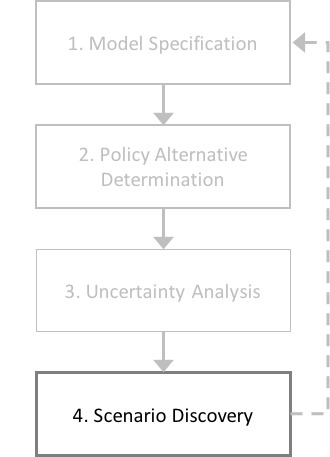
\includegraphics{structure-step4}
    \caption{RDM Structure - Step 4}
    \label{fig:structure-step4}
\end{figure}

\newpage

\section{Scenario Discovery Theory} \label{step4-scenariodiscovery}
The fundamental goal of scenario discovery is to determine which characteristics of a problem, including uncertainty and policy lever settings, lead to specific outcome behaviors \citep{Bryant2010}. When only a small number of scenarios are being considered at a time, it is easier to see patterns and determine which elements of those scenarios lead to a specific outcome behavior without further processing or cleaning. However, given the rise of computer-aided experimentation, the number of scenarios and policies considered can increase dramatically \citep{Lempert2008}. In the case of an RDM-based analysis, 10,000 or more scenarios can be considered, along with tens or even hundreds of policy options. This makes it impossible to detect patterns that affect system behavior. 

Scenario discovery within an RDM-based method aims to develop easy to understand descriptions of which areas of the uncertainty space remain vulnerable, despite searching for policy alternatives that are meant to be the most successful \citep{Kasprzyk2013}. This typically involves statistical and data-mining algorithms to discover patterns in a set of data. The two most commonly recognized scenario discovery algorithms are CART, a classification algorithm, and PRIM, a bump-hunting algorithm \citep{Lempert2008}. Research that has compared the two algorithms has discovered that while both PRIM and CART generally result in similar information, PRIM provides more opportunity for interaction and requires less initial configuration for the analyst \citep{Bryant2010}. Because of this, PRIM will be used for this analysis. 

\subsection{Patient rule induction method (PRIM)}
PRIM, also known as the Patient Rule Induction Method, uses a bump-hunting algorithm to identify a range of values that best predict the behavior of a subset of cases from the entire data set that fail to meet a specific goal \citep{Friedman1999}. To accomplish this, PRIM optimizes along three different axes: density, coverage, and interpretability, and attempts to maintain an even balance between density and coverage. Density refers to the fraction of cases in an identified cluster in which failure is recognized; coverage concerns the fraction of identified failure cases that are contained within that cluster; interpretability incorporates the ease with which users are able to understand what is discovered by the algorithm \citep{Lempert2013}. 

The algorithm involves initial configuration, followed by a series of two iterative and interactive steps that search for any common elements that correspond to a specific behavior of interest. 

\begin{enumerate}[leftmargin=*]
    \item Determine which experiments are of interest. This generally involves a classification mechanism in which experiments that lead to one or more outcomes of interest which doesn't meet a specific threshold. This can be, for example, the robustness thresholds specified in the configuration of the domain criterion metric in \cref{step0-robust}. 
    \item Search for regions
    \begin{enumerate}
        \item The algorithm constructs a series of boxes that are increasingly smaller and denser by slowly restricting the input space based on the removal of a small subset of elements that will lead to the greatest increase of the mean inside that new box. This step concludes with a series of boxes known as a "peeling trajectory" \citep{Lempert2008}
        \item The peeling trajectory is presented to the analyst, who is able to select one or more of the boxes that most effectively balances goals of having high density and high coverage \citep{Lempert2008}. These boxes are known as candidate boxes. Candidate boxes describe the ranges of various input parameters (whether that be uncertainties, decision levers, or both) that describe the behavior found in each box. 
        \item The analyst is able to restart the process to construct a new series of boxes. The algorithm will remove all data sets that are included in the first series and start again. The process can repeat until the analyst has discovered all useful information and ends the search. 
    \end{enumerate}
\end{enumerate}

%TODO describe this algorithm in more detail, including sample peeling trajectories....?

\section{Implementation Details} \label{step4-implementation}
PRIM has been implemented as an open-source algorithm using many different languages, including R and Python, making it easy to use; this analysis specifically will leverage the Python-based implementation found in the EMA-Workbench \citep{Kwakkel2016SD}.

This implementation of PRIM for this study involves developing a binary classification of the cases of interest, where 1 indicates that case should be considered by the PRIM algorithm, and a 0 means it does not include the behavior of interest and should therefore be ignored. Case classification will consider each outcome separately by selecting cases that do not meet the robustness threshold as defined in \cref{step0-robust} for each outcome of interest. Analysis will consider uncertainties and decision levers as drivers of behavior both separately and together.

Again, scenario discovery is executed for each set of non-dominated policy alternatives. This means that during multi-scenario MORDM, the scenario discovery process is run independently for each selected reference scenario. 
